where $N_t=\sum_{j=t-W+1}^{t}\mathbf{1}_{\{\mathrm{Burn}_j>0\}}$ is the count of positive-burn months in the window.

\subsection{Break-even and Reserve}
\paragraph{Operational and cash break-even (first month that satisfies).}
\begin{align}
t^{\mathrm{BE\_op}} 
  &= \min\{\, t \mid \mathrm{MRR}^{\mathrm{rec}}_t \ge C^{\mathrm{monthly}}_t \,\},\\
t^{\mathrm{BE\_cash}} 
  &= \min\{\, t \mid \Pi_t \ge 0 \,\}.
\end{align}

\paragraph{Cumulative burn to cash break-even and reserve.}
\begin{align}
\mathrm{Burn}^{\mathrm{cum}}_{\le t^{\mathrm{BE\_cash}}} 
  &= \sum_{j=1}^{t^{\mathrm{BE\_cash}}} \max\{0,\ -\Pi_j\},\\
\mathrm{Reserve}
  &= \text{INITIAL\_CAPITAL} - \mathrm{Burn}^{\mathrm{cum}}_{\le t^{\mathrm{BE\_cash}}}.
\end{align}

\subsection{Policy Gates (Spend \& Acquisition Multipliers)}
\paragraph{Spend gate (applied to next month’s cost).}
With guardrail $R_{12}$ months and spend cut $\gamma$:
\begin{align}
s_t 
  &= 
  \begin{cases}
    1-\gamma, & \mathrm{Runway}_{t-1} < R_{12},\\
    1, & \text{otherwise.}
  \end{cases}
\end{align}

\paragraph{PLG soft-freeze (applied to current month acquisitions).}
With soft-freeze threshold $R_{9}$ months:
\begin{align}
m^{\mathrm{PLG}}_t 
  &= 
  \begin{cases}
    0.7, & \mathrm{Runway}_{t-1} < R_{9},\\
    1, & \text{otherwise.}
  \end{cases}
\end{align}

\subsection{Mapping from Code to Symbols (for clarity)}
\begin{itemize}
  \item $P_{\mathrm{ent}} = \texttt{PRICES['enterprise\_mrr']}$, $P_p=\texttt{PRICES['standard'|'business'|'scale']}$, $P_{\mathrm{pod}}=\texttt{PRICES['add\_on\_pod']}$.
  \item $\delta_{\mathrm{PLG}}=\texttt{CHURN\_PLG\_MONTHLY}$, $\delta^{\mathrm{annual}}_{\mathrm{SLG}}=\texttt{CHURN\_SLG\_ANNUAL}$.
  \item $r_p,\ \bar{n}_p$ from \texttt{ADD\_ON\_ADOPTION[plan]['adoption\_rate'|'avg\_pods']}.
  \item $\rho,\ \bar{u},\ P_{\mathrm{store}}$ from \texttt{STORE\_REVENUE}.
  \item $a^p_y$ from \texttt{ACQUISITION\_PLG[y]} tuples; $A^{\mathrm{SLG}}_y$ from \texttt{ACQUISITION\_SLG[y]}.
  \item $u_k$ from \texttt{UPLIFT} and $\mathrm{Cost}_{k,y}$ from the respective cost dictionaries.
  \item $s_t$ controlled by \texttt{SPEND\_CUT\_PERCENTAGE} and \texttt{RUNWAY\_GUARDRAIL}
  \item $m^{\mathrm{PLG}}_t$ controlled by \texttt{ACQ\_DAMPING\_WHEN\_SOFT\_FREEZE} and \texttt{RUNWAY\_SOFT\_FREEZE}.
\end{itemize}

GitHub link \href{https://github.com/kuduk/intellyhub-businessplan/blob/main/breakeven.v2.02.py}{Python Script Model}

\newpage
\subsection{Break-even Analysis: Chart}
\begin{figure}[H]
    \centering 
    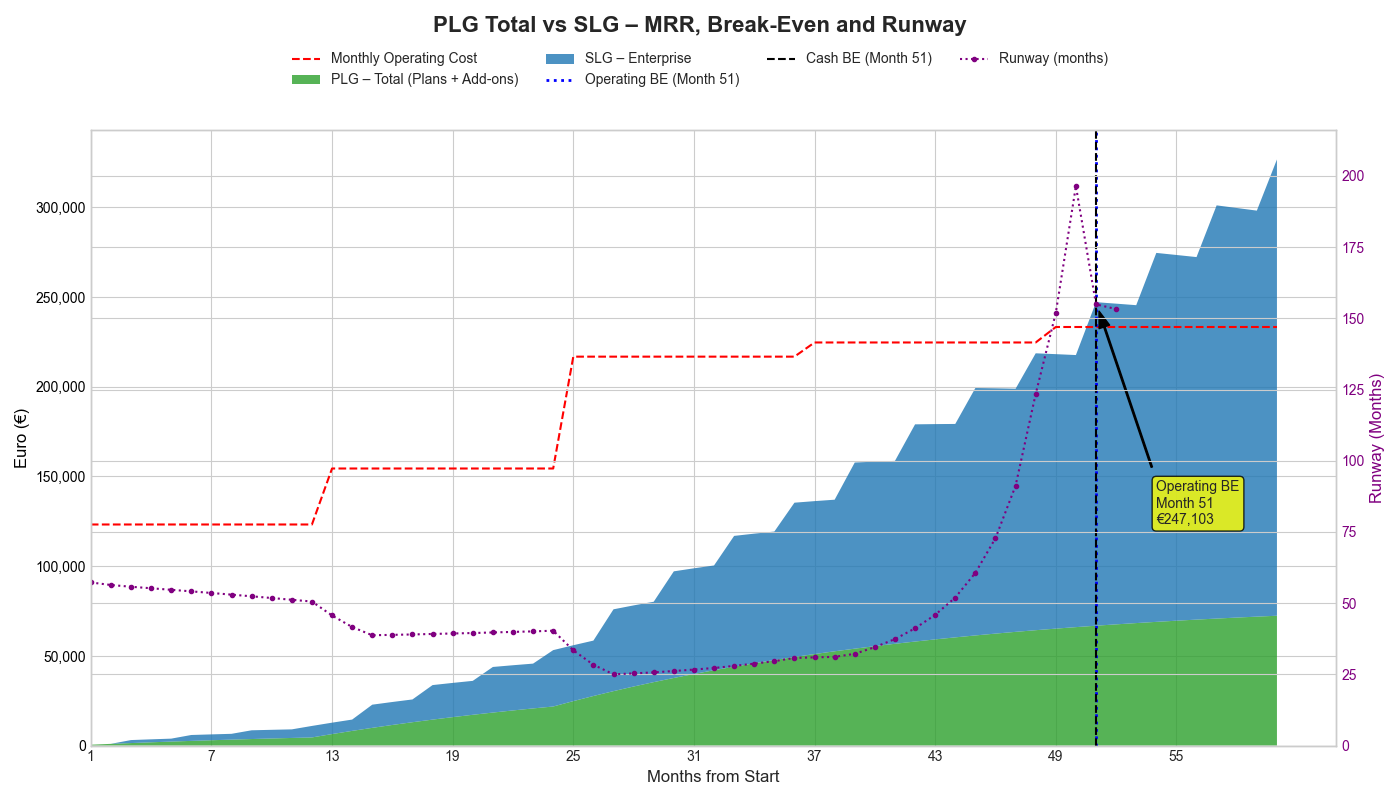
\includegraphics[width=\textwidth]{financial_projection.png}
    \caption{Break-even analysis: PLG vs. SLG MRR, monthly costs, and runway.}
    \label{fig:break_even_analysis}
\end{figure} 
\subsection{Break-even Analysis: Chart Interpretation}

\paragraph{Legend (quick read)}
\begin{itemize}
  \item \textbf{Green (PLG -- Plans + Add-ons):} self-service recurring revenue.
  \item \textbf{Blue (SLG -- Enterprise):} enterprise recurring revenue; grows in quarterly ``steps'' because annual deals are smoothed across quarters.
  \item \textbf{Red dashed:} monthly operating cost (with prudential uplifts), rising in yearly steps.
  \item \textbf{Purple dotted:} runway (months), computed as cash divided by the 3-month moving average burn.
  \item \textbf{Vertical lines:} operational break-even (blue, month~51) and cash break-even (black, month~51).
\end{itemize}

In the first three years the chart shows a patient build. The green PLG area rises steadily as monthly sign-ups compound (after churn) and add-ons add incremental MRR. The blue SLG area climbs in visible quarterly steps when enterprise contracts are booked. Costs move in blocks: each new year adds planned capacity (teams, infra, G\&A with uplifts), so the red line jumps and then stays flat until the next step.

These dynamics match the year-end figures. At the end of year~1, costs are \textbf{€123{,}212}/month versus \textbf{€10{,}948}/month of recurring MRR (loss \textbf{€112{,}149}/month, cash \textbf{€5{,}740{,}147}, runway \textbf{50.6} months). By year~2: \textbf{€154{,}413} vs.\ \textbf{€53{,}194} (loss \textbf{€100{,}855}/month), cash \textbf{€4{,}282{,}549}, runway \textbf{40.3} months. By year~3: \textbf{€216{,}746} vs.\ \textbf{€135{,}360} (loss \textbf{€80{,}631}/month), cash \textbf{€2{,}239{,}361}, runway \textbf{30.8} months. The curve of revenues clearly closes the gap to costs while cash remains controlled: the \textbf{minimum observed runway is 25.0 months} and the \textbf{peak monthly burn} is \textbf{€160{,}442}.

In year~4 the gap narrows decisively. The larger SLG steps make the blue area expand faster and the stack (PLG+SLG) nearly meets the cost line. Year-end: costs \textbf{€224{,}646}/month versus recurring MRR \textbf{€218{,}614}/month (total revenue \textbf{€219{,}615}/month), a near-flat loss of \textbf{€5{,}031}/month, cash \textbf{€2{,}239{,}361}. The purple runway line starts to spike because the moving-average burn approaches zero.
